\apendice{Especificación de diseño}

\section{Introducción}

En este apartado se describe el diseño general del sistema desarrollado, explicando cómo se organizan internamente los distintos componentes y cómo se gestionan los datos dentro de Blender.

El sistema se divide en dos addons que trabajan conjuntamente:

\begin{itemize}
    \item Un addon de captura de datos, encargado de detectar y registrar eventos mientras el usuario trabaja dentro de Blender.
    
    \item Un addon de análisis y visualización, utilizado para procesar la información registrada y generar métricas y representaciones visuales.
\end{itemize}

La comunicación de ambos add-ons se efectúa mediante archivos CSV lo que implica que la etapa de registro puede estar ajena a la fase de evaluación. Esta organización proporciona mayor flexibilidad en cuanto a mantenimiento y simplifica el crecimiento futurista en la creación de nuevas versiones.

El diseño consideró tanto los principios del modularismo como la separación de funciones para asegurar que cada parte del software tuviera su propósito específico dentro del sistema. La sección estuvo dividida en tres aspectos fundamentales: diseño de información, diseño arquitectónico y diseño procedimental.

\section{Diseño de datos}

El sistema persiste los datos en archivos CSV como medio principal. Estos archivos albergan las transacciones registradas durante la interacción del usuario con Blender, lo que permite que se procesen posteriormente por el addon analítico.

Se ha elegido un enfoque orientado a eventos para la gestión de datos, ya que cada registro refleja un hecho significativo ejecutado por el usuario en el ámbito de la modelización.

Cada registro en la base de datos es equivalente a un evento identificado por el sistema. La base de datos contiene datos temporales, identificativos, espaciales y geométricos; esta información proporciona un completo vistazo del estado de la escena a la hora del evento.

Un ejemplo sencillo de registro producido por el sistema sería:

\begin{verbatim}
USER_ID,TimeStamp,UserX,UserY,UserZ,
VertexDelta,ModeChanged,ShiftD,Merge

b3cef250,1777534745.32,7.51,-2.6,3.96,
-8,0,0,0
\end{verbatim}

Cada registro almacena información temporal, espacial y geométrica relacionada con el estado de la escena y las acciones realizadas por el usuario durante la sesión de modelado.

\begin{table}[H]
\centering
\small
\begin{tabular}{l l}
\hline
\textbf{Campo} & \textbf{Descripción} \\
\hline
USER\_ID & Identificador del usuario \\
TimeStamp & Marca temporal del evento \\
UserX,Y,Z & Posición del usuario en la escena \\
VertexDelta & Cambio en el número de vértices \\
ModeChanged & Cambio de modo en Blender \\
ShiftD & Detección de duplicado \\
Merge & Operación de unión de geometría \\
\hline
\end{tabular}
\caption{Ejemplo de campos registrados en los archivos CSV.}
\label{tab:csv_fields}
\end{table}

Esta estructura facilita tanto el análisis automatizado como la evaluación manual de los registros de información.

La Figura~\ref{fig:diseno_datos} muestra la estructura lógica de los datos gestionados por el sistema.

\begin{figure}[H]
    \centering
    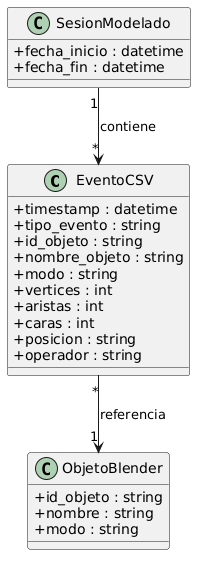
\includegraphics[height=0.85\textheight, keepaspectratio]{diagramas/diseno_datos.png}
    \caption{Estructura lógica de los datos registrados por el sistema.}
    \label{fig:diseno_datos}
\end{figure}

De forma general, cada evento incluye los siguientes campos:

\begin{itemize}
    \item \textbf{timestamp}: marca temporal exacta del evento.
    \item \textbf{tipo\_evento}: tipo de acción registrada.
    \item \textbf{id\_objeto}: identificador único del objeto afectado.
    \item \textbf{nombre\_objeto}: nombre asignado al objeto dentro de la escena.
    \item \textbf{modo}: modo de trabajo activo en el momento del evento.
    \item \textbf{propiedades}: conjunto de atributos geométricos y contextuales relevantes.
\end{itemize}

Además de los datos capturados por el primer addon, el segundo addon genera estructuras derivadas destinadas al cálculo de métricas y a la generación de visualizaciones.

Entre los datos procesados por el sistema de análisis se incluyen:

\begin{itemize}
    \item Métricas temporales.
    \item Estadísticas de interacción.
    \item Valores normalizados para representación gráfica.
    \item Coordenadas para generación de geometría visual.
\end{itemize}

El formato CSV respeta los parámetros de sencillez, compatibilidad y capacidad de procesamiento para obtener datos mediante análisis automático o verificación directa.

Asimismo, la Figura~\ref{fig:diseno_componentes} representa el sistema desde el punto de vista de componentes software.

\begin{figure}[H]
    \centering
    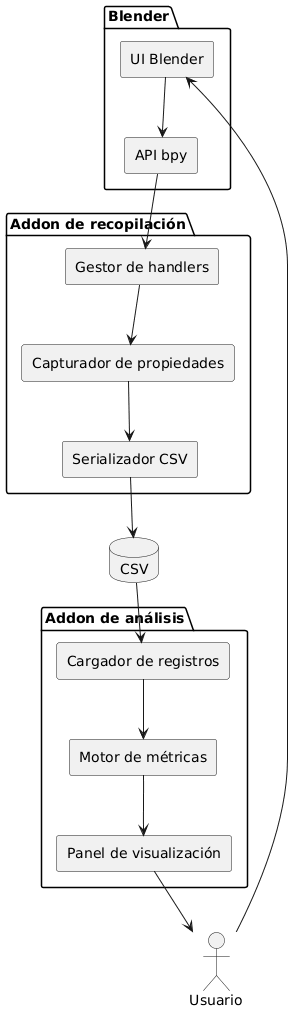
\includegraphics[height=0.85\textheight, keepaspectratio]{diagramas/diseno_componentes.png}
    \caption{Diagrama de componentes del sistema.}
    \label{fig:diseno_componentes}
\end{figure}

\subsection{Addon de recopilación de datos}

El primer addon se encarga de monitorizar la interacción del usuario dentro de Blender.

Sus principales responsabilidades son:

\begin{itemize}
    \item Detectar eventos mediante \textit{handlers}.
    \item Identificar operaciones realizadas sobre objetos.
    \item Capturar información geométrica y contextual.
    \item Registrar eventos en archivos CSV.
\end{itemize}

El sistema hace uso de los \textit{handlers} de Blender para ejecutar funciones automático al detectar modificaciones en la escena.

\begin{verbatim}
bpy.app.handlers.depsgraph_update_post.append(operator_tracker)
\end{verbatim}

Este enfoque facilita un seguimiento constante del estado de la escena sin la intervención del usuario necesario.

Este componente opera de forma invisible para el usuario y está diseñado para optimizar la performance del entorno de modelado.

Para reducir la carga informativa guardada, el sistema evita recoger datos durante las sesiones en las que no se registran cambios pertinentes.

\begin{verbatim}
if not state_changed and not any_operator_flag:
    return None
\end{verbatim}

Gracias a esta estrategia se disminuye considerablemente la cantidad de datos redundantes generados durante las sesiones de modelado.

Además, el sistema genera firmas simplificadas del estado de la escena para detectar modificaciones importantes entre actualizaciones consecutivas.

\begin{verbatim}
signature = (verts, ngons, tris, mode, uv_hash)
\end{verbatim}

Estas firmas permiten comprobar rápidamente si el estado de la escena ha cambiado antes de registrar nueva información.

\subsection{Addon de análisis y visualización}

El segundo addon actúa como una capa de procesamiento y representación visual sobre los datos registrados por el primer componente.

Sus funciones principales incluyen:

\begin{itemize}
    \item Lectura y procesamiento de archivos CSV.
    
    \item Cálculo de métricas temporales, espaciales y estructurales.
    
    \item Generación de gráficos estadísticos.
    
    \item Creación de visualizaciones tridimensionales dentro de Blender.
    
    \item Integración de herramientas externas como \textit{matplotlib}.
\end{itemize}

El sistema se organizó en distintos módulos para separar las responsabilidades principales y facilitar el mantenimiento del código.

La Figura~\ref{fig:interna} muestra los distintos componentes internos del addon.

\begin{figure}[H]
    \centering
    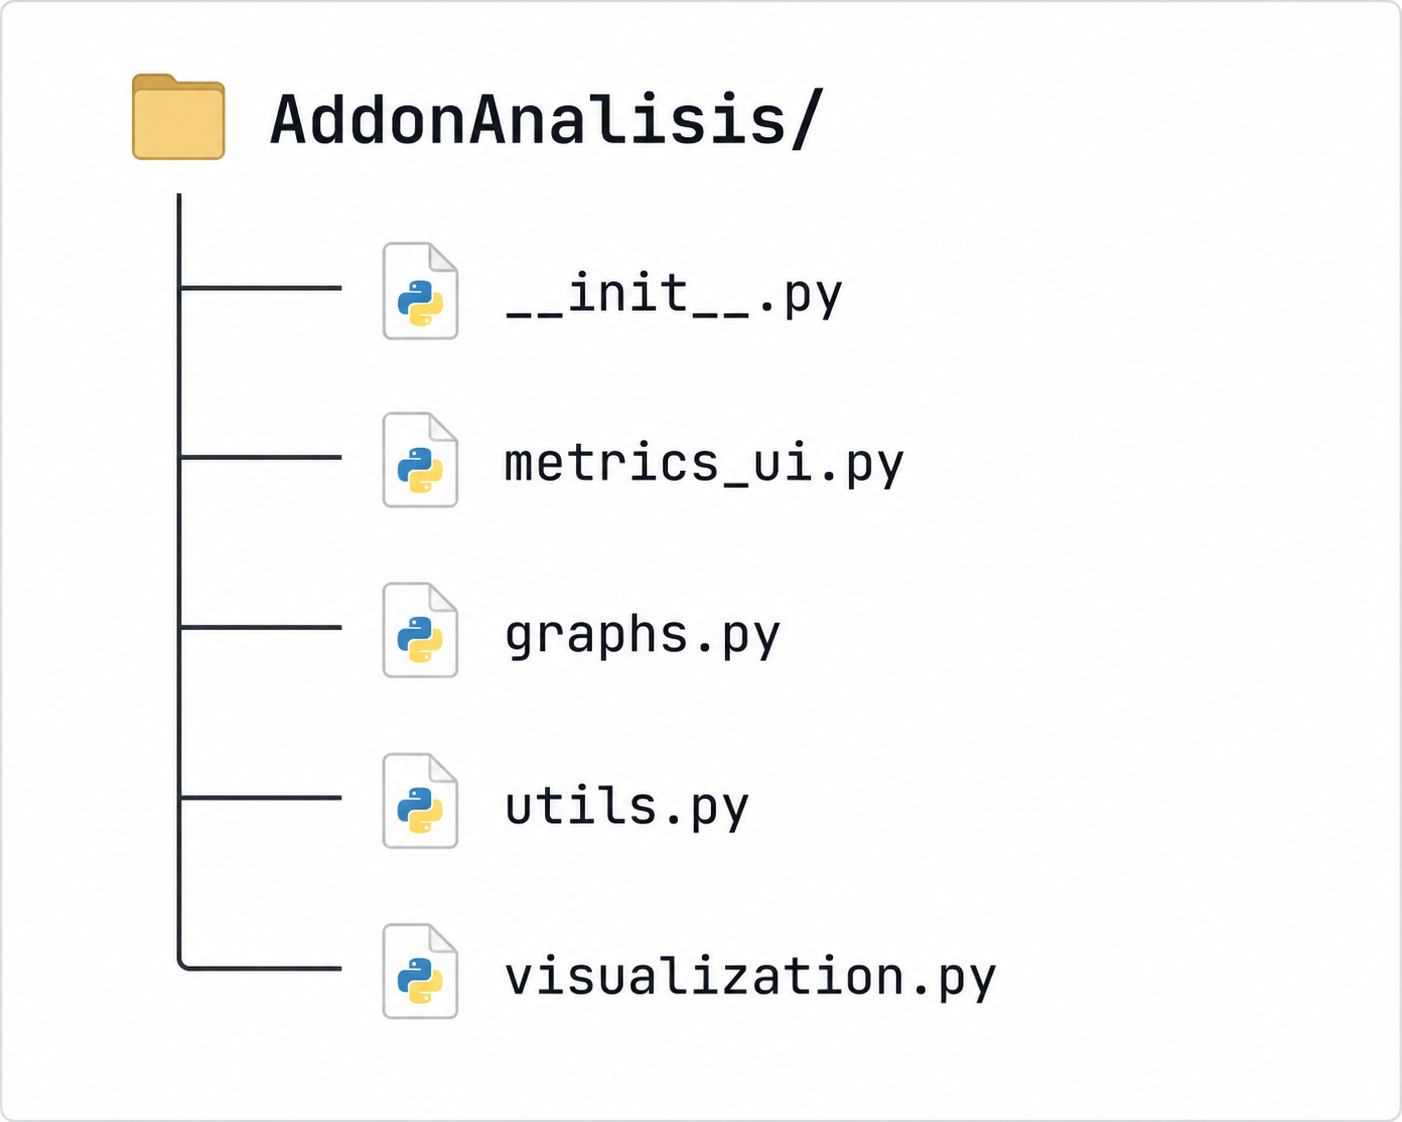
\includegraphics[height=0.85\textheight, keepaspectratio]{diagramas/interna.png}
    \caption{Diagrama de componentes del sistema.}
    \label{fig:interna}
\end{figure}

Algunos de los archivos más importantes utilizados durante el desarrollo fueron:

\begin{itemize}
    \item \texttt{metrics\_ui.py}: controla la interfaz principal y las opciones de análisis.
    
    \item \texttt{graphs.py}: genera gráficos y representaciones visuales dentro de Blender.
    
    \item \texttt{utils.py}: incluye funciones auxiliares relacionadas con el cálculo y procesamiento de métricas.
    
    \item \texttt{\_\_init\_\_.py}: registra y conecta los distintos componentes internos del addon.
\end{itemize}

Las métricas se generan automáticamente en base a los datos que se capturan durante la sesión de modelado.

\begin{verbatim}
ANALYSIS[metric_id]["label"]
\end{verbatim}

Esto permite organizar las métricas de forma más flexible y agruparlas según el tipo de análisis que se quiera realizar.

Para generar gráficos temporales y representaciones estadísticas se utilizaron librerías externas como \textit{matplotlib}.

\begin{verbatim}
plt.plot(x, y)
plt.show()
\end{verbatim}

Este tipo de representaciones facilita analizar visualmente la evolución de distintas métricas durante el modelado.

Se generan parte de las visualizaciones del sistema dentro del entorno 3D de Blender mediante geometría procedurales.

\begin{verbatim}
bpy.ops.mesh.primitive_cube_add(location=(x, y, z))
\end{verbatim}

Esto también permite mostrar las métricas como objetos tridimensionales dentro de la escena original, lo que facilita un mejor análisis y comprensión de los datos de manera visual.||copia|Una parte de

El sistema también puede modificar propiedades visuales de los objetos en función de los valores calculados durante el análisis.

\begin{verbatim}
obj.scale = (value, value, value)
\end{verbatim}

Esto permite representar visualmente diferencias entre métricas utilizando tamaño, posición u otras propiedades espaciales.

Este componente permite representar la información analítica directamente dentro del entorno tridimensional, facilitando la interpretación de los datos.

\subsection{Comunicación entre addons}

La comunicación entre ambos addons se realiza mediante archivos CSV intermedios.

Utilizar archivos CSV como punto de conexión entre ambos addons permitió simplificar bastante el flujo de trabajo del sistema y facilitó las tareas de depuración y análisis.

La arquitectura modular permite que ambos componentes evolucionen de forma independiente, manteniendo una integración coherente dentro del sistema global.

\section{Diseño procedural}

El diseño procedural explica la secuencia de pasos realizados por el sistema en respuesta al acto del usuario.

Figura~\ref{fig:diseno_procedimental} ilustra la secuencia fundamental del funcionamiento del sistema.

\begin{figure}[H]
    \centering
    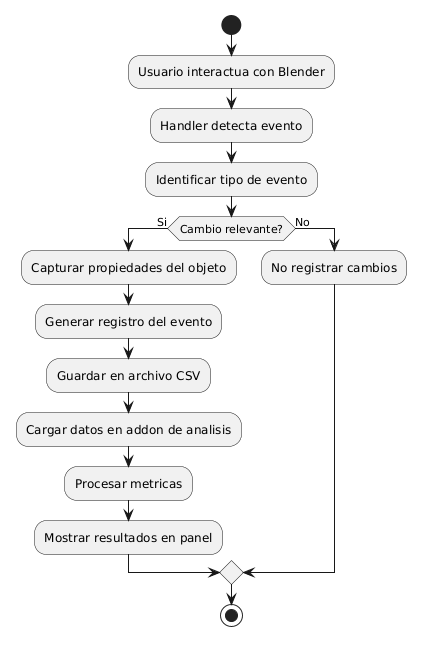
\includegraphics[width=0.65\textwidth]{diagramas/diseno_procedimental.png}
    \caption{Flujo procedimental del sistema.}
    \label{fig:diseno_procedimental}
\end{figure}

La Figura~\ref{fig:diseno_secuencia} representa la interacción temporal entre los distintos componentes.

\begin{figure}[H]
    \centering
    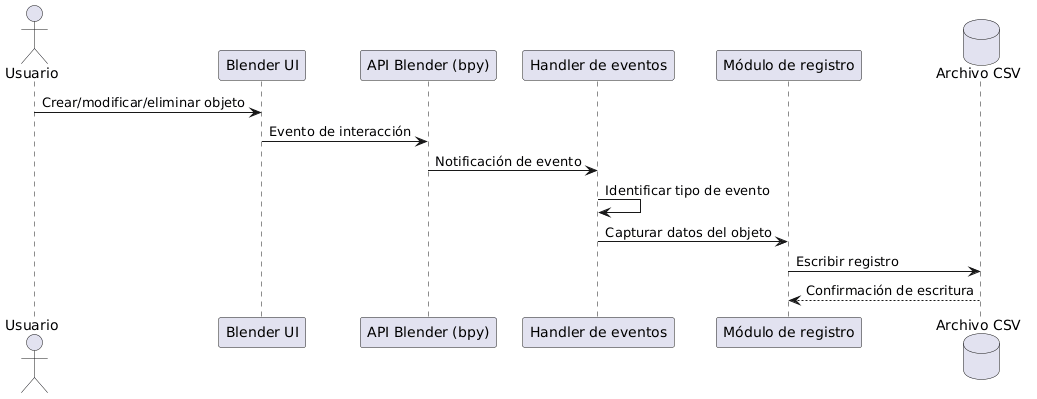
\includegraphics[width=0.85\textwidth]{diagramas/secuencia.png}
    \caption{Diagrama de secuencia del sistema.}
    \label{fig:diseno_secuencia}
\end{figure}

Todo el funcionamiento del sistema se ejecuta automáticamente mientras el usuario trabaja de manera habitual dentro de Blender.

El flujo general de ejecución es el siguiente:

\begin{enumerate}
    \item El usuario realiza una acción en Blender.
    \item El sistema detecta el evento mediante \textit{handlers} registrados.
    \item Se identifican el tipo de acción y el objeto afectado.
    \item Se capturan las propiedades relevantes del estado de la escena.
    \item Se genera un registro estructurado del evento.
    \item El registro se almacena en el archivo CSV correspondiente.
    \item El addon de análisis carga y procesa los datos registrados.
    \item Se calculan métricas y estadísticas.
    \item El sistema genera visualizaciones gráficas o tridimensionales.
    \item Los resultados se muestran dentro de Blender.
\end{enumerate}

El sistema optimiza el rendimiento evitando registrar información redundante y almacenando únicamente cambios significativos en el estado de los objetos.

\section{Decisiones de diseño relevantes}

Durante el desarrollo del sistema se adoptaron diversas decisiones clave que condicionan su estructura y comportamiento.

\begin{itemize}

    \item \textbf{Separación en dos addons}: permite desacoplar completamente la captura de datos del análisis y visualización, facilitando la modularidad y el mantenimiento.

    \item \textbf{Uso de CSV como formato de persistencia}: proporciona una solución ligera, interoperable y fácilmente depurable.

    \item \textbf{Captura basada en handlers}: permite detectar automáticamente eventos en Blender sin intervención directa del usuario.

    \item \textbf{Procesamiento diferido de métricas}: evita sobrecargar el sistema durante la captura de datos.

    \item \textbf{Registro selectivo de cambios}: reduce significativamente el volumen de información generada y mejora la eficiencia.

    \item \textbf{Visualización integrada en Blender}: permite representar métricas directamente dentro del entorno de modelado.

    \item \textbf{Uso de librerías externas}: permitió incorporar gráficos y representaciones estadísticas utilizando herramientas como \textit{matplotlib}.

\end{itemize}

Todas estas decisiones ayudaron a desarrollar un sistema más organizado, flexible y fácil de ampliar en futuras versiones del proyecto.

Por último, la Figura~\ref{fig:arquitectura} muestra una visión general del sistema completo, integrando ambos addons y el flujo de información entre ellos.

\begin{figure}[H]
 \centering
 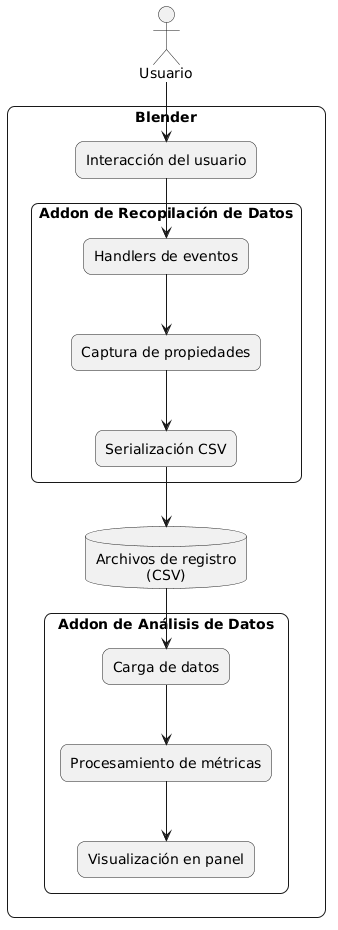
\includegraphics[height=0.85\textheight, keepaspectratio]{diagramas/diseno_arquitectura_vertical.png}
 \caption{Arquitectura global del sistema basada en dos addons complementarios.}
 \label{fig:arquitectura}
\end{figure}
